\documentclass{article}

\usepackage{caption}
\usepackage{graphicx}
\usepackage{float}
\usepackage{enumitem}
\usepackage{hyperref}

\begin{document}
	\section{Cell cycle}
	
	\begin{enumerate}[label=\textbullet]
		\item Cyclin-Dependent Kinases (CDKs) phosphorylate proteins that drive the cell through the cell cycle
		\item Cyclines activate the CDKs (partially)
	\end{enumerate}
	
	\begin{table}[h]
		\centering
		\begin{tabular}{|c|c|c|} \hline
			Cyclin & Cdks & Complex \\ \hline
			Cyclin-D & (Cdk4/Cdk6)  & G1-Cdk \\ \hline
			Cyclin-E & Cdk2         & G1/S-Cdk \\ \hline
			Cyclin-A & (Cdk2/Cdk1)  & S-Cdk (MPF) \\ \hline
			Cyclin-B & Cdk1         & M-Cdk (MPF)\\ \hline
		\end{tabular}
		\caption{Cyclines and the Cdks they form complexes with}
	\end{table}

	The resulting complex when Cyclin A or B bind to Cdk1/Cdk2 is called the maturation promoting factor (MPF). In its inactive form, the cdk is phosphorylated and the Cyclin dephosphorylated and both are dissociated. After reversing these states, they form the MPF which then triggers chromosome condensation, disbanding of the nuclear envelope and organisation of the spindle apparatus.\\
	Cdk concentration remains mostly constant.\footnote{albert, p. 1093} Concentration of cyclins changes during the cell cycle (see images).
	
	\begin{figure}[H]
		\centering
		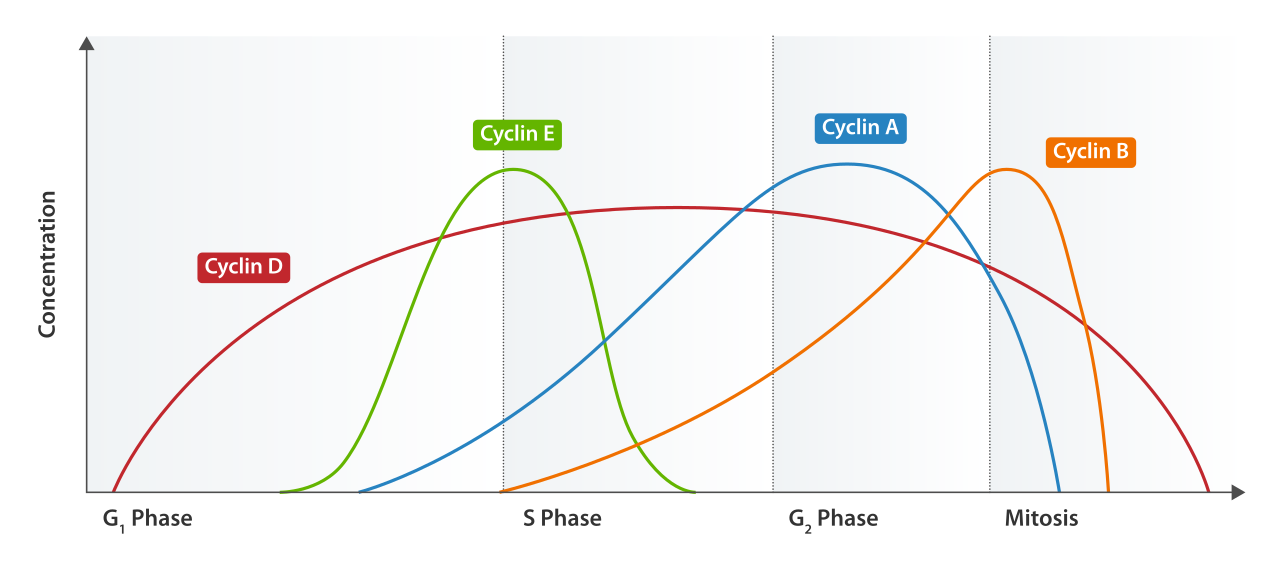
\includegraphics[width=\linewidth]{cyclin_activity_wikipedia.png}
		\caption{Concentration of the cyclins during the cell cycle (wikipedia)}
	\end{figure}

	\begin{figure}[H]
		\centering
		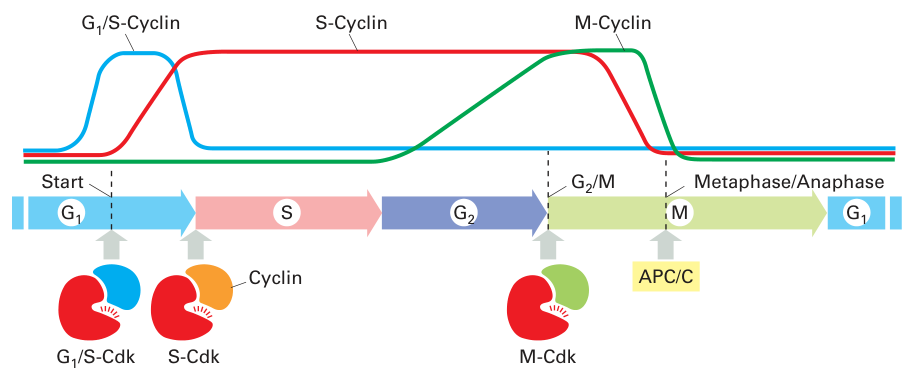
\includegraphics[width=\linewidth]{cyclin_activity_alberts.png}
		\caption{Concentration of the cyclins during the cell cycle (alberts)}
	\end{figure}

	\begin{figure}[H]
		\centering
		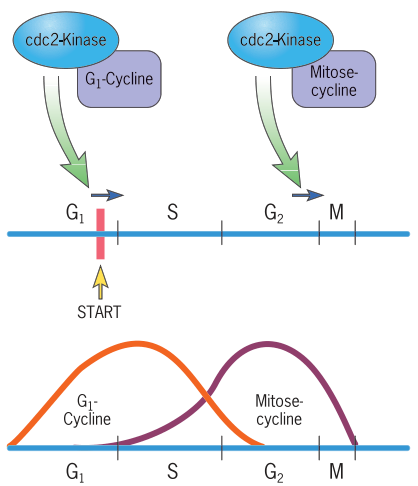
\includegraphics[width=0.8\linewidth]{cyclin_activity_karp.png}
		\caption{Concentration of the cyclins during the cell cycle (karp). cdc2 = cdk1}
	\end{figure}
	
	\begin{enumerate}[label=\textbullet]
		\item G1/S-Cdk initiates the cell cycle in the dormant G1 phase 
		\begin{enumerate}[label=\textbullet]
			\item S-Cdk triggers transition from the G1 to the S phase 
			\item M-Cdk triggers transition from the G2 to the M phase 
		\end{enumerate}
		
		\item CDK-activating kinase (CAK) activates any Cyclin-Cdk complex by phosphorylation
		\item Cyclin-dependent kinase inhibitor protein (CKI) inhibits Cyclin-Cdk complexes by binding to them (mostly G1/S- and S-Cdks)
		
		\item Wee1 inhibits Cyclin-Cdk complexes by phosphorylation, causing a delay of the M-Phase so that the cell can grow. If Wee1 is defective, the cells transition directly from S- to M-Phase without the growth in the G2 phase, resulting in \textit{wee} little cells :)
		\item Cdc25 reverses that inhibition by dephosphorylation
		
		\item The anaphase-promoting complex/cyclosome (APC/C) triggers transition from the metaphase to the anaphase by ubiquitylation of securin and Cyclin-A/Cyclin-B, marking them for proteolysis
		\begin{enumerate}[label=\textbullet]
			\item APC/C binds with Cdc20 (Mitosis) or Cdh1 (late Mitosis-G1) to identify target proteins 
		\end{enumerate}
		
		\item SCF ubiquitylates CKIs in the late G1 phase, thus activating S-Cdks; it's also responsible for proteolysis of G1/S-Cdks in the early S phase
		\item SCF is regulated by its F-Box subunits, which can only bind specifically phosphorylated proteins 
	\end{enumerate}

	\begin{figure}[H]
		\centering
		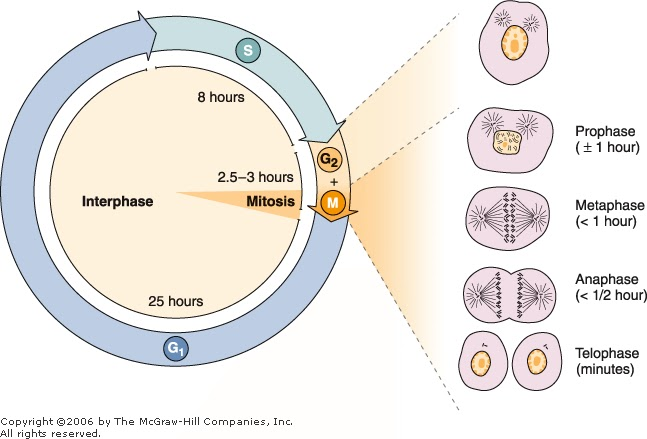
\includegraphics[width=0.8\linewidth]{durations.jpg}
		\caption{\url{https://dehistology.blogspot.com/2011/06/cell-cycle.html}}
	\end{figure}

\end{document}